\section{Segurança de Redes}

\subsection{O que é segurança de rede?}

    \begin{itemize}[left=0.5cm, align=left, nosep]    
        \item \textbf{Confidencialidade:} Apenas o emissor e o receptor pretendido devem “entender” o conteúdo da mensagem.
        \begin{itemize}[left=0.5cm, nosep, label=$\hookrightarrow$]
            \item Emissor: \underline{criptografa} a mensagem
            \item Receptor: \underline{descriptografa} a mensagem
        \end{itemize} 
        \item \textbf{Autenticação:} O emissor e o receptor desejam confirmar a identidade um do outro.
        \item \textbf{Integridade da mensagem:} O emissor e o receptor desejam garantir que a mensagem não foi alterada 
        (durante a transmissão ou depois) sem detecção.
        \item \textbf{Acesso e disponibilidade:} Os serviços devem ser acessíveis e disponíveis para os usuários.
    \end{itemize}  

    \textbf{Exemplo}
    \begin{itemize}[left=0.5cm, align=left, nosep] 
        \item Bob e Alice (amantes!) querem se comunicar ``com segurança''
        \item Trudy (intrusa) pode interceptar, apagar e adicionar mensagens
    \end{itemize}
        
    \begin{figure}[H]
        \centering
        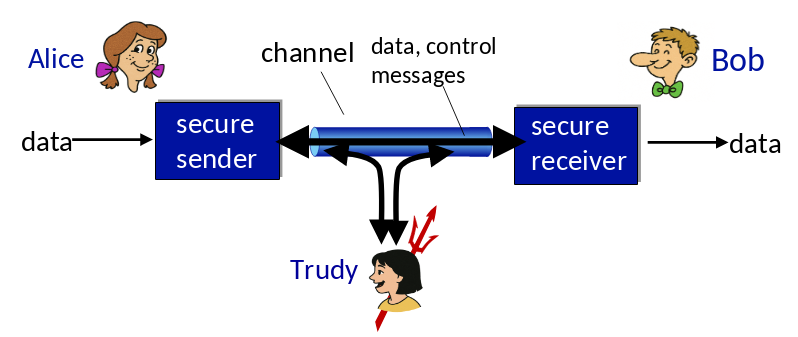
\includegraphics[width=0.75\textwidth]{img/exemplo.png}
    \end{figure}

    Alice e Bob podem ser:
    \begin{itemize}[left=0.5cm, align=left, nosep] 
        \item Navegador web/servidor para transações eletrônicas (ex: compras online)
        \item Cliente/servidor de banco online
        \item Servidores DNS
        \item Roteadores BGP trocando atualizações de tabelas de roteamento
    \end{itemize}

    Trudy, o ``bad guy'' pode ser:
    \begin{itemize}[left=0.5cm, align=left, nosep] 
        \item \textbf{Eavesdrop:} Interceptar mensagens.
        \item Inserção \textbf{ativa} de  mensagens em uma conexão.
        \item \textbf{Impersonation:} Pode falsificar (\textit{spoof}) o endereço de origem no pacote (ou qualquer campo do pacote).
        \item \textbf{Hijacking:} ``Assumir'' uma conexão em andamento removendo o emissor ou o receptor e inserindo-se no lugar.
        \item \textbf{Denial of service:} Impedir que o serviço seja usado por outros (ex: sobrecarregando recursos).
    \end{itemize}

\subsection{Princípios da criptografia}

    \begin{figure}[H]
        \centering
        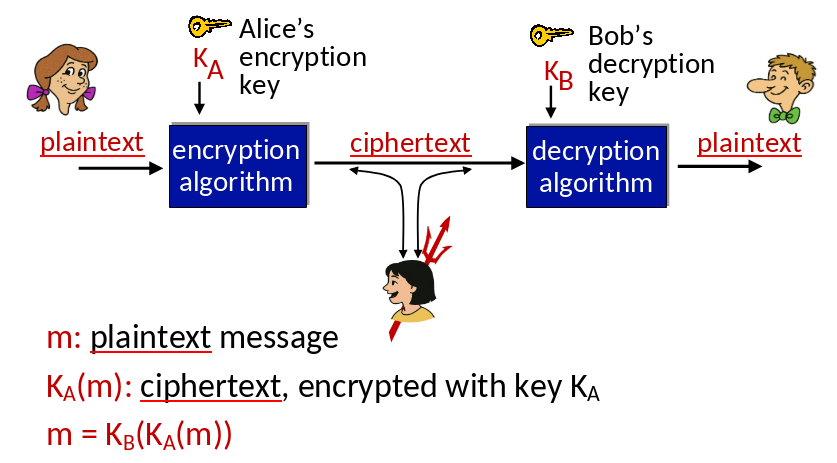
\includegraphics[width=0.75\textwidth]{img/criptografia.png}
    \end{figure}

    \textbf{Quebrando um esquema de criptografia}

    \begin{itemize}[left=0.5cm, align=left, nosep]    
        \item \textbf{Ataque somente com texto cifrado (cipher-text only attack):} Trudy possui apenas o \underline{texto cifrado} (ciphertext) para analisar.
        \item \textbf{Duas abordagens:}
        \begin{itemize}[left=0.5cm, nosep, label=$\hookrightarrow$]
            \item Força bruta: Testar todas as chaves possíveis
            \item Análise estatística
        \end{itemize}  
        \item \textbf{Ataque com texto conhecido (known-plaintext attack):} Trudy possui o \underline{texto original} (plaintext) correspondente ao \underline{texto cifrado} 
        (ciphertext).
        \begin{itemize}[left=0.5cm, nosep, label=$\hookrightarrow$]
            \item Ex: Em uma cifra monoalfabética, Trudy determina associações para a, l, i, c, e, b, o
        \end{itemize} 
        \item \textbf{Ataque com texto escolhido (chosen-plaintext attack):} Trudy pode obter o \underline{texto cifrado} (ciphertext) a partir de textos que ela mesma escolhe.
    \end{itemize}  

    \textbf{Criptografia com chave simétrica}

    \begin{figure}[H]
        \centering
        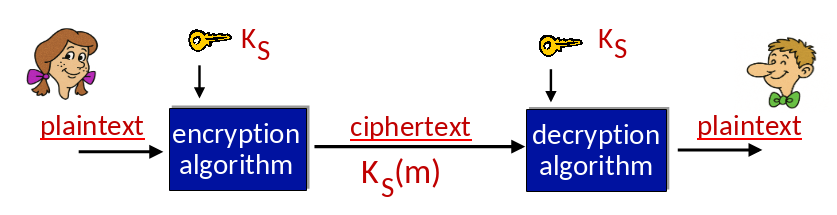
\includegraphics[width=0.65\textwidth]{img/criptografia-simetrica.png}
    \end{figure}

    \begin{itemize}[left=0.5cm, align=left, nosep]    
        \item \textbf{Criptografia de chave \underline{simétrica}:} Bob e Alice compartilham a mesma chave (simétrica): K.
        \begin{itemize}[left=0.5cm, nosep, label=$\hookrightarrow$]
            \item Ex: A chave consiste em conhecer o padrão de substituição em uma cifra de substituição monoalfabética.
        \end{itemize}  
    \end{itemize}  

    \textbf{Esquema de criptografia simples}    
    \begin{itemize}[left=0.5cm, align=left, nosep]    
        \item \textbf{Cifra de substituiçãos (substitution cipher):} Substitui um elemento por outro.
        \begin{itemize}[left=0.5cm, nosep, label=$\hookrightarrow$]
            \item Cifra \underline{monoalfabética}: Substitui uma letra por outra.
        \end{itemize}  
    \end{itemize}  
    
    \begin{figure}[H]
        \centering
        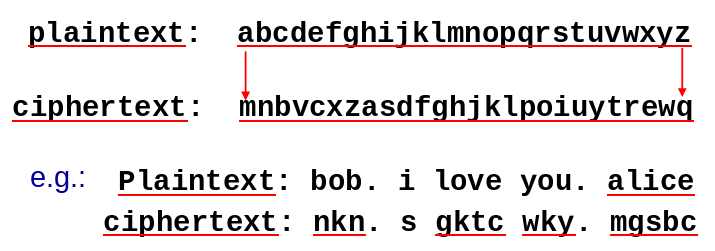
\includegraphics[width=0.65\textwidth]{img/esquema-de-criptografia.png}
    \end{figure}

    \begin{itemize}[left=0.5cm, align=left, nosep]    
        \item \textbf{Chave de criptografia:} Mapeamento de um conjunto de 26 letras para outro conjunto de 26 letras.
    \end{itemize}
    
    \textbf{Esquema de criptografia sofisticada}
    \begin{itemize}[left=0.5cm, align=left, nosep]    
        \item $n$ cifras de substituição: $M_1, M_2,\ldots, M_n$
        \item Padrão cíclico:
        \begin{itemize}[left=0.5cm, nosep, label=$\hookrightarrow$]
            \item e.g, $n = 4$: $M_1, M_3, M_4, M_3, M_2$; $M_1, M_3, M_4, M_3, M_2$; \ldots
        \end{itemize}     
        \item Para cada novo símbolo do \underline{texto original}, utiliza-se o próximo padrão de substituição no ciclo.
        \begin{itemize}[left=0.5cm, nosep, label=$\hookrightarrow$]
            \item e.g, dog: d: $M_1$; o: $M_3$; g: $M_4$.
        \end{itemize} 
        \item \textbf{Chave de criptografia:} $n$ cifras de substituição e o padrão cíclico.
        \begin{itemize}[left=0.5cm, nosep, label=$\hookrightarrow$]
            \item A chave não precisa ser apenas um padrão de $n$ bits.
        \end{itemize} 
    \end{itemize}  

    \textbf{Criptografia de chave simétrica: DES}
    \begin{itemize}[left=0.5cm, align=left, nosep]    
        \item \textbf{DES (Data Encryption Standard):}
        \begin{itemize}[left=0.5cm, nosep, label=$\hookrightarrow$]
            \item Padrão de criptografia dos EUA [NIST 1993].
            \item Chave simétrica de 56 bits, entrada de \underline{texto original} (plaintext) de 64 bits.
            \item Cifra de bloco com encadeamento de blocos (cipher block chaining).
        \end{itemize}     
        
        \item Quão seguro é o DES  
        \begin{itemize}[left=0.5cm, nosep, label=$\hookrightarrow$]
            \item \textbf{DES Challenge:} Uma frase criptografada com chave de 56 bits foi \underline{descriptografada} (por força bruta) em menos de um dia.
            \item Não há ataques analíticos eficazes conhecidos.
        \end{itemize} 
        
        \item Tornando o DES mais seguro:
        \begin{itemize}[left=0.5cm, nosep, label=$\hookrightarrow$]    
            \item \textbf{3DES:} Criptografa 3 vezes com 3 chaves diferentes.
        \end{itemize}
    \end{itemize}  

    \textbf{AES: Padrão de Criptografia Avançada (Advanced Encryption Standard)}
    \begin{itemize}[left=0.5cm, align=left, nosep]    
        \item Padrão de \textbf{chave simétrica} do NIST, que substituiu o DES (novembro de 2001)
        \item Processa dados em \underline{blocos de 128 bits}.
        \item Utiliza chaves de \underline{128, 192 ou 256 bits}.
        \item A descriptografia por \underline{força bruta} (testando cada chave), que leva cerca de 1 segundo no DES, levaria aproximadamente 149 trilhões de anos no AES-128. 
    \end{itemize}  
    
    \textbf{Criptografia de Chave Pública (Public Key Cryptography)}
    \begin{itemize}[left=0.5cm, align=left, nosep]    
        \item \textbf{Criptogrfia com chave simétrica:}
        \begin{itemize}[left=0.5cm, nosep, label=$\hookrightarrow$]
            \item Exige que o emissor e o receptor conheçam uma chave secreta \textbf{compartilhada}.
            \item Como estabelecer essa chave, se nunca se emcontraram ?  
        \end{itemize}
        \item \textbf{Criptografia de chave pública:}
        \begin{itemize}[left=0.5cm, nosep, label=$\hookrightarrow$]
            \item Abordagem radicalmente diferente ([Diffie-Hellman76, RSA78])
            \item Emissor e receptor \textbf{não compartilham} uma chave secreta.
            \item Chave \textbf{pública} de \underline{criptografia}: conhecida por \textbf{todos}.
            \item Chave \textbf{privada} de \underline{descriptografia}: conhecida apenas pelo \textbf{receptor}.   
        \end{itemize}
 
        \begin{figure}[H]
        \centering
            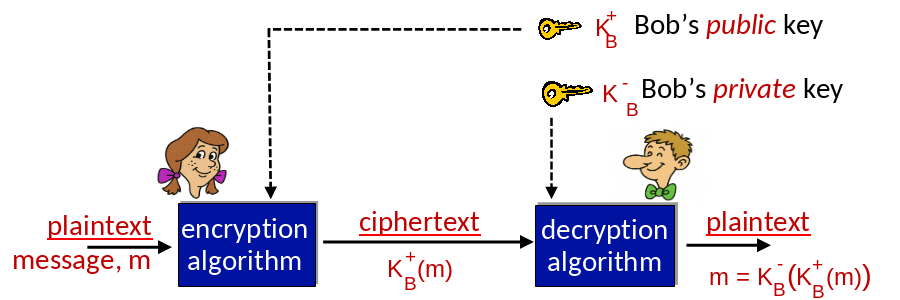
\includegraphics[width=0.65\textwidth]{img/criptografia-chave-publica.png}
        \end{figure}

        \item \textbf{Observação:} A criptografia de chave pública revolucionou um campo de 2000 anos (que antes utilizava apenas criptografia simétrica).
        \begin{itemize}[left=0.5cm, nosep, label=$\hookrightarrow$]
            \item Ideias semelhantes surgiram aproximadamente na mesma época, de forma independente nos EUA e no Reino Unido (inicialmente classificadas).
        \end{itemize}

    \end{itemize}  

    \textbf{Algoritmos de criptografia de chave pública}
    \begin{itemize}[left=0.5cm, align=left, nosep]    
        \item \textbf{Algoritmo de criptografia:} É o \underline{método} ou conjunto de regras matemáticas usado para transformar um texto em forma ilegível.    
        \begin{itemize}[left=0.5cm, nosep, label=$\hookrightarrow$]
            \item Exemplos: AES, RSA, DES.
        \end{itemize}          
        \item \textbf{Chave de criptografia:} É um \underline{valor secreto} utilizado pelo algoritmo para realizar a criptografia e a descriptografia.  
        \item \textbf{Analogia:}
        \begin{itemize}[left=0.5cm, nosep, label=$\hookrightarrow$]
            \item Algoritmo: tipo de cadeado.
            \item Chave: chave que abre o cadeado.
        \end{itemize}
        
        \item Requisitos:
        \begin{enumerate}[left=0.5cm, align=left, nosep]
            \item É necessário ter $K_{b}^{+}(\bullet) \text{ e } K_{b}^{-} (\bullet)$ tal que $K_{b}^{-} (K_{b}^{+} (m)) = m$.
            \item Dada a chave pública $K_{b}^{+}$ deve ser impossível calcular/computar a chave privada $K_{b}^{-}$. 
        \end{enumerate}
    
        \item \textbf{RSA (Rivest-Shamir-Adleman):} O algoritmo de criptografia de chave pública mais amplamente utilizado.
    \end{itemize}  

    \textbf{Pré-requisito: Aritmética Modular}
    \begin{itemize}[left=0.5cm, align=left, nosep]    
        \item $x \bmod n =$ resto de $x$ quando dividido por $n$.   
        \item \textbf{Propriedades:} \\
        $[(a \bmod n) + (b \bmod n)] \bmod n = (a + b) \bmod n$ \\
        $[(a \bmod n) - (b \bmod n)] \bmod n = (a - b) \bmod n$ \\
        $[(a \bmod n) \cdot (b \bmod n)] \bmod n = (a \cdot b) \bmod n$ 
        \item Assim, $(a \bmod n)^{d}  \bmod n = a^d \bmod n$
        \item \textbf{Exemplo:} $x = 14, n = 10, d = 2$: \\
        $(x \bmod n)^{d} \bmod n = 4^{2} \bmod 10 = 16 \bmod 10 = 6$; \\
        $x^{d} = 14^{2} = 196; x^{d} \bmod 10 = 6$ 
    \end{itemize}

    \textbf{RSA: Conceitos Básicos}
    \begin{itemize}[left=0.5cm, align=left, nosep]    
        \item \textbf{Mensagem:} É apenas um \underline{padrão} de bits.
        \item Um \underline{padrão de bits} pode ser representado de forma \textbf{única} por um \underline{número inteiro}.
        \item Assim, criptografar uma mensagem é equivalente a criptografar um número.
        \item Exemplo: 
        \begin{itemize}[left=0.5cm, nosep, label=$\hookrightarrow$]
            \item $m = 10010001$. Essa mensagem é representada de forma \textbf{única} pelo número decimal $145$.
            \item Para criptografar $m$, criptografamos o número correspondente, o que gera um \underline{novo número} (o \underline{texto cifrado}).
        \end{itemize}
    \end{itemize}

    \textbf{RSA: Criação do par de chaves pública/privada}
    \begin{enumerate}[left=0.5cm, align=left, nosep]
        \item Escolher dois \underline{números primos} grandes $p$ e $q$ (por exemplo, 1024 bits cada).
        \item Calcular $\mathbf{n} = pq$ e $z = (p-1)(q-1)$.
        \item Escolher $\mathbf{e}$ (com $e < n$) tal que não possua \underline{fatores comuns} com $z$ (ou seja, $e$ e $z$ são \underline{coprimos}).
        \item Escolher $\mathbf{d}$ tal que $ed - 1$ seja exatamente \underline{divisível} por $z$ (ou seja, $ed \bmod z = 1$).
       \item A chave \textbf{pública} é $\underbrace{(\mathbf{n}, \mathbf{e})}_{K_b^+}$ e a chave \textbf{privada} é $\underbrace{(\mathbf{n}, \mathbf{d})}_{K_b^-}$.
    \end{enumerate}
    
    \textbf{RSA: Criptografia e Descriptografia}
    \begin{enumerate}[left=0.5cm, align=left, nosep]
        \item Dados $(\mathbf{n}, \mathbf{e})$ e $(\mathbf{n}, \mathbf{d})$ como calculados anteriormente.
        \item Para criptografar uma mensagem $m$ ($m < n$), calcular: $c = m^e \bmod n$.
        \item Para \underline{descriptografar} o padrão de bits recebido $c$, calcular: $m = c^d \bmod n$.
    \end{enumerate}

    \[
    m = \left(\underbrace{m^e \bmod n}_{c}\right)^d \bmod n
    \]

    \textbf{Exemplo:} 
    Bob escolhe: $p = 5, q = 7$. Então, $n = 35$ e $z = 24$. \\
    $e = 5$ (Assim, $e$ e $z$ são relativamente coprimos). \\
    $d = 29$ (Assim, $ed - 1$ é divisível por $z$, ou seja, $ed \bmod z = 1$). \\
    Criptografando mensagens de 8 bits. 
    \begin{figure}[H]
        \centering
        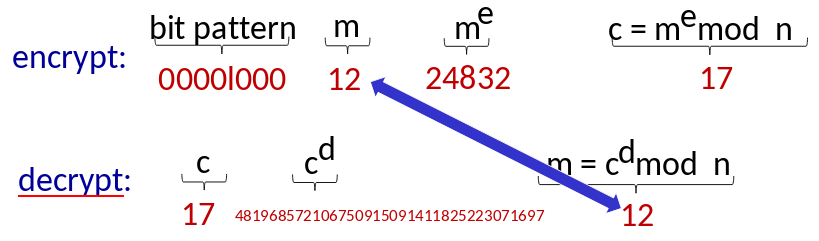
\includegraphics[width=0.65\textwidth]{img/exemplo-rsa.png}
    \end{figure}

    \textbf{Por que o RSA funciona?}

    \begin{enumerate}[left=0.5cm, align=left, nosep]
        \item Deve-se mostrar que: $c^d \bmod n = m,\text{onde } c = m^e \bmod n$.
        \item Fato: para quaisquer $x$ e $y$: $x^{y} \bmod n = x^{(y \bmod n)} \bmod n$
        \begin{itemize}[left=0.5cm, nosep, label=$\hookrightarrow$]
            \item Onde $n = pq$ e $z = (p-1)(q-1)$
        \end{itemize} 
        \item Então, 
        \[
        \begin{aligned}
            c^d \bmod n &= (m^e \bmod n)^d \bmod n \\
            &= m^{ed} \bmod n \\
            &= m^{(ed \bmod z)} \bmod n \\
            &= m^{1} \bmod n \\
            &= m
        \end{aligned}
        \]
    \end{enumerate}

    \textbf{RSA: Outra Propriedade Importante}
    \[
    \begin{aligned}
        \underbrace{K_B^{-}(K_B^{+}(m))}_{\substack{\text{Usa uma chave pública,} \\ \text{seguida por uma privada}}} = m = 
        \underbrace{K_B^{+}(K_B^{-}(m))}_{\substack{\text{Usa uma chave privada,} \\ \text{seguida por uma pública}}}
    \end{aligned}
    \]

    \begin{itemize}[left=0.5cm, align=left, nosep]
        \item Isso acontece diretamente da aritmética modular.
    \end{itemize}
    \[
    \begin{aligned}
    (m^e \bmod n)^d \bmod n &= m^{ed} \bmod n \\
                            &= m^{de} \bmod n \\
                            &= (m^d \bmod n)^e \bmod n
    \end{aligned}
    \]

    \textbf{Por que o RSA é seguro?}

    \begin{itemize}[left=0.5cm, align=left, nosep]
        \item Se você conheçe a chave pública de Bob $(n, e)$. Quão difícil é determinar $d$?
        \item Essencialmente, é necessário encontrar os fatores de $n$ sem conhecer previamente os dois fatores $p$ e $q$.
        \begin{itemize}[left=0.5cm, nosep, label=$\hookrightarrow$]
            \item Fato: fatorar um número grande é computacionalmente difícil.
        \end{itemize}
    \end{itemize}

    \textbf{RSA na prática: chaves de sessão}
    \begin{itemize}[left=0.5cm, align=left, nosep]
        \item A exponenciação no RSA é computacionalmente intensiva.
        \item O DES é pelo menos 100 vezes mais rápido que o RSA.
        \item Utiliza-se \underline{criptografia} de chave pública para estabelecer uma \textbf{conexão segura} e, em seguida, define-se uma segunda chave — a chave de 
        sessão simétrica — para criptografar os dados; chave de sessão: $K_S$.
        \item Bob e Alice usam RSA para trocar uma \textbf{chave de sessão} simétrica $K_S$.
        \item Aós ambos possuírem $K_S$, utilizam criptografia de \underline{chave simétrica}.
    \end{itemize}
